\documentclass[a4paper, 12pt]{article}
\usepackage{graphicx}

\usepackage[utf8]{inputenc}
\usepackage[magyar]{babel}

% a szép matematikai szimbólumokért
\usepackage{amssymb}
\usepackage{amsmath}

% ha táblázatban szeretnénk egyesített sorokat is
\usepackage{multirow}

% horizontal line
\usepackage{hhline}

% eps formátumú ábrák --> pdflatex fordításhoz!!
\usepackage{epsfig}

% egyenletekhez, pl mátrixok írására
\usepackage{array}

% ha betűszíneket is szeretnénk használni
\usepackage{color}

% Margók egyéni beállításai
\usepackage{anysize}
\marginsize{1.64cm}{1.64cm}{1.2cm}{2.4cm} %\left right top bottom

% vakszöveg
\usepackage{lipsum}
\usepackage{blindtext}

% A HIVATKOZÁSOKHOZ HASZNÁLT CSOMAGOK. RÉSZLETESEBBEN LD: google -> latex bibtex
\usepackage[numbers, square, comma, sort&compress]{natbib}
%\usepackage[format=hang,labelsep=period]{caption}

\usepackage[unicode]{hyperref}   % ezzel a hivatkozások linkké válnak
\usepackage{bookmark}
\hypersetup{bookmarksopen={true}}
\hypersetup{bookmarksopenlevel={2}}
\hypersetup{bookmarksnumbered={true}}
\hypersetup{
	colorlinks,%
	citecolor=red,%
	filecolor=black,%                                                                                                                                               
	linkcolor=blue,%
	urlcolor=green
}
\numberwithin{equation}{section}          % ezekkel tudod beállítani, hogy milyen felbontásig menjen a hivatkozás
\numberwithin{figure}{subsection}
%\numberwithin{table}{section}          % ha kikommenteled, akkor csak simán számozva lesz.

%%%%%%%%%%%%%%%% Néhány dolog a fancy kinézethez

\frenchspacing
\setlength{\parskip}{2ex}
\setlength{\headsep}{0,4cm}
\setlength{\headheight}{4pt}

% fej- es lábléc
\usepackage{fancyhdr}
\usepackage{fancyref}
\usepackage{fancyvrb}
\pagestyle{fancy}

\renewcommand{\headrulewidth}{0,05pt}
\renewcommand{\footrulewidth}{0pt}


\fancyhf{}
\fancyhead[RE]{{ \nouppercase{\leftmark}} }
\fancyhead[LO]{{ \nouppercase{\leftmark}} }
\cfoot{--~\thepage~--}


%%%%%%%%%%%%%%%%%%%%%%%%%%%%%%%%%%%%%%%%%%%%%%%%%%%%%%%%%%%%%%%%%%%%%%%%%%%%%%%%%%%%%%%%
%%%%%%%%%%%%%%%%%%%%%%%%%%%%%%%%%%%%%%%%%%%%%%%%%%%%%%%%%%%%%%%%%%%%%%%%%%%%%%%%%%%%%%%%

\begin{document}
	
	% Címoldalt lehet egyszerűen a \maketitle paranccsal is. Ha kissé részletesebb
	% címre van szükség, azt lehet így is, kézzel megadva mindent.
	\begin{titlepage}   
		
		\begin{center}
			
			\thispagestyle{empty}  
			
			\vspace*{1.5cm}

			{\LARGE Geometriai Brown-mozgás \\ és pénzügyi modellezés }

			\vspace*{1.5cm}
			
			{\small ,,A kutatómunka információs eszközei" \\
				tárgyra készült hallgatói dokumentáció}
			
			\vspace*{1.5cm}

			{\footnotesize Írta: Bóna Márton} \\
			{\footnotesize ver.: 2018.04.17.}
			
			\vspace*{3cm}

			\begin{figure}[h!]
				\begin{center}
					
\includegraphics[width=0.5\textwidth]{D:/ADAT/github/algo_trad_rand_walk/documents/img/elte.eps}
				\end{center}
			\end{figure}
			
		\end{center}
	
	\end{titlepage}
	
	\newpage
	
	%%%%%%%%%%%%%%%%%%%%%%%%%%%%%%%%%%%%%%%%%%%%%%%%%%%%%%%%%%%%%%%%%%%%%%%%%%%%%%%%%%%%%%%%
	  
	\thispagestyle{empty}
	
	\begin{abstract}
		
		Ezen dokumentum ,,A kutatómunka információs eszközei" tárgyra készített programozási
		eszközök megismerése céljából létrehozott beadandó dokumentációja.
		
		A dokumentum röviden összefoglalja a tárgy elvárását a beadandóval kapcsolatban,
		továbbá ismerteti a kiválasztott probléma alapjait. A feladatot párfős csapatoknak
		kell megoldaniuk, így szó fog esik a csapatmunkáról és a feladatok szétosztásáról.
		Továbbiakban a saját feladatrészem munkafolyamatát és a fejlesztés során adódó problémák
		megoldásáról fogok írni. Végezetül bemutatásra kerül a végeredmény.

	\end{abstract}
	
	% ---------------------------- T A R T A L O M J E G Y Z É K ----------------------------
	
	\newpage \vspace*{2cm}
	\thispagestyle{plain}                                                                                                                                             
	\pagenumbering{roman} \setcounter{page}{1}
	\tableofcontents
	
	\clearpage \vspace*{2cm}
	\thispagestyle{plain}
	\listoffigures
	
	\pagenumbering{arabic} \setcounter{page}{1}
	\thispagestyle{fancy}
	\clearpage
	
	% ---------------------------- M A G A   A   D O L G O Z A T ----------------------------
	
	%%%%%%%%%%%%%%%%%%%%%%%%%%%%%%%%%%%%%%%%%%%%%%%%%%%%%%%%%%%%%%%%%%%%%%%%%%%%%%%%%%%%%%%%

	\section{Bevezetés}
	\markboth{Bevezetés}{}
	
		A pénzügyi modellezésben használt elméletek tesztelésére, továbbá
		különböző gazdasági szituációk előállítására régóta használnak sztochasztikus folyamaton
		alapuló árfolyammodelleket.
		
		Ezen árfolyammodellek lényege, hogy minden lépésben egy valószínűségi változótól függ,
		hogy milyen irányba és mekkorát változik az árfolyam, ezáltal lehetőség nyílik
		arra, hogy sok adaton tudjuk tesztelni elméleteinket.
		Az egyik használható sztochasztikus folyamat a geometriai Brown-mozgás.
		A geometriai Brown-mozgást a következő sztochasztikus differenciálegyenlet írja le.
		
		\begin{equation}
		dS(t) = \mu S(t) dt + \sigma S(t) dB(t)
		\end{equation}
	
		Ahol $S(t)$ jelöli például egy részvény árát $t$ időpillanatban, $\mu$ az úgynevezett \textit{drift} paraméter, $\sigma$ pedig a \textit{volatilitás} paraméter.
		A drift alatt azt kell érteni, hogy hosszú távon az árfolyam milyen irányba fog változni,
		volatilitás alatt pedig az árfolyam rövidtávú változékonyságát kell érteni, nagy 
		volatilitás esetén az árfolyam rövid idő alatt nagy kilengéseket produkálhat.
		
		$B(t)$-ről még nem beszéltünk, ez szintén egy sztochasztikus folyamat értéke adott
		időpillanatban, ez a folyamat pedig nem más mint a Wiener-folyamat, más nevén standard
		Brown-mozgás. A Wiener-folyamat ismérve, hogy értékének két időpillanat közötti változásai 
		függetlenek egymástól és normális eloszlást követnek nulla várható értékkel és $dt$
		szórásnégyzettel.
		
		\begin{figure}[h!]
			\begin{center}
				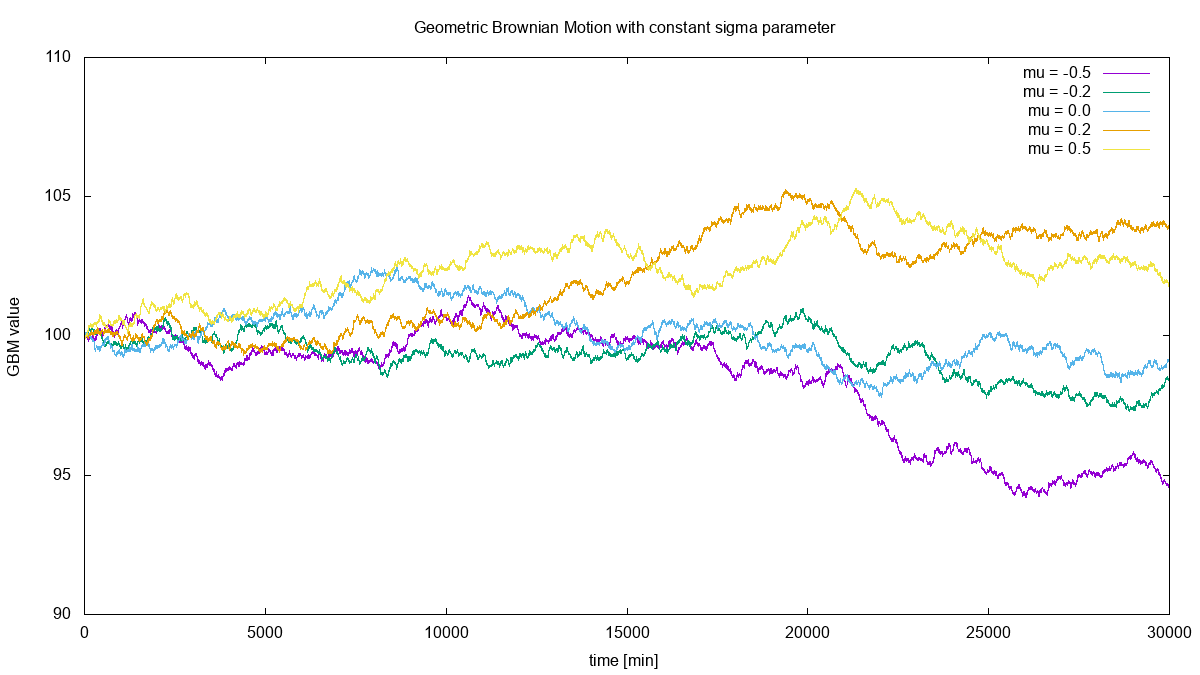
\includegraphics[width=0.9\textwidth]{D:/ADAT/github/algo_trad_rand_walk/documents/plot/GBM_data_plot/const_sigma.png}
			\end{center}
			\caption{GBM adott $\sigma$ és öt különböző $\mu$ értékkel}
			\label{fig:gbm}
		\end{figure}
		
		Az \ref{fig:gbm} ábrán jól látható, hogy a drift paraméter tényleg befolyással van
		a hosszútávú árfolyam alakulásra. Az említett sztochasztikus folyamatokról bővebben
		\cite{brown} és \cite{geobrown} Wikipédia oldalakon lehet olvasni.
		
	%%%%%%%%%%%%%%%%%%%%%%%%%%%%%%%%%%%%%%%%%%%%%%%%%%%%%%%%%%%%%%%%%%%%%%%%%%%%%%%%%%%%%%%%
	
	\clearpage
	
	\section{A feladat}
	\markboth{A feladat}{}
	
		\subsection{A kitűzött feladat}
	
		A feladat az volt, hogy keressünk egy témát, amelyhez kapcsolhatók programozási feladatok
		,majd osszuk fel egymás között a választott feladatokat. Mindenkinek implementálni kell
		egy programot, ami végrehajtja a kitűzött elvárást és ezen programokat egy megfelelő
		struktúrába rendezve létre kell hozni egy automatikus fordítási környezetet. Azaz 
		a programhoz kapcsolható bemeneti és kimeneti fájlokat, generált képeket és a dokumentáció 
		függőségeit rögzíteni kell, hogy egyszerű parancs kiadásával minden legyártódjon,
		Majd végül a feladatot és a tapasztalatokat rögzíteni kell a jelen dokumentációban.
		
		Megoldandó feladatnak egy pénzügyi programcsomag összeállítását választottuk.
		Létre kellet hozni egy programot ami képes árfolyamot generálni, majd ezeken az
		adatokon alapvető gazdasági indikátorok segítségével pénzügyi kereskedést valósít meg.
		Végül a kereskedés eredményét és a legyártott árfolyamokat ábrázolni kell.

		%%%%%%%%%%%%%%%%%%%%%%%%%%%%%%%%%%%%%%%%%%%%%%%%%%%%%%%%%%%%%%%%%%%%%%
	
		\subsection{A feladatok felosztás}
		
		A csapat négy tagú volt és különböző programozási nyelvhez értettünk.
		Ezért úgy döntöttünk, hogy két nyelvet használunk. Ketten közülünk python
		nyelven dolgoztak, az egyikük a feladat kereskedés részét valósította meg,
		a másikuk pedig az eredmények és az árfolyamok ábrázolását.
		A másik kétfős egység, amiben én voltam, c++ nyelvet használt és két
		sztochasztikus folyamaton alapuló árfolyammodellt hozott létre, melyből az adatokat
		a másik kétfős csapat használta fel. A két árfolyammodell a Wiener-folyamaton és a
		geometriai Brown-mozgáson alapul.
		
		Az én feladatom volt a geometriai Brown-mozgás implementálása c++ nyelven. A továbbiakban
		erről írok majd, de előbb még szót ejtek hogyan valósult meg a csapatmunka.
		
	%%%%%%%%%%%%%%%%%%%%%%%%%%%%%%%%%%%%%%%%%%%%%%%%%%%%%%%%%%%%%%%%%%%%%%%%%%%%%%%%%%%%%%%%
	
	\section{Csapatmunka}
	%\markboth{Csapatmunka}{}
	
		A csapat vezetését én vállaltam el. Kezdetben több személyes találkozón megbeszéltük,
		hogy ki milyen nyelven tud programozni, és ennek függvényében választottunk egy feladatot
		, amely felosztható megfelelő alegységekre. Ezután tisztáztuk, hogy pontosan kinek mi
		a feladata és a feladatrészek hogyan függenek egymástól.
		Megbeszéltük, hogy milyen kommunikációs csatornán folytatjuk a további egyeztetéseket.
		A feladat verziókövetését és a csapatmunkát a git (github) környezet segítségével oldottuk
		meg. A projekt github elérhetősége \cite{gitrepo}.
		
		A csoportvezetés során a github környezet felállítását, az alap könyvtárszerkezetet és
		a munkafolyamtok követését én végeztem. A CMake fájlok inicializálását szintén én végeztem.
		
		Továbbá a csapat számár egy github bevezető jegyzetet és gyakorlófeladatot is készítettem,
		hogy a szintén kezdő csapatársak könnyeben el tudják sajátítani a munkához szükséges
		ismereteket.
	
	%%%%%%%%%%%%%%%%%%%%%%%%%%%%%%%%%%%%%%%%%%%%%%%%%%%%%%%%%%%%%%%%%%%%%%%%%%%%%%%%%%%%%%%%
	
	\section{Saját feladatrész}
	\markboth{Saját feladatrész}{}
	
		\subsection{Alapgondolatok}
	
		Miután közösen megbeszéltük kinek mi a feladata és megértettük a git alapjait,
		nekiálltam a saját alfeladatomnak.
		
		A feladatom a geometriai Brown-mozgás implementálása c++ programozási nyelven,
		továbbá adatok (árfolyamok) gyártása a többiek számára feldolgozáshoz.
		Az előbbiből következik, hogy egy jól általánosított programot érdemes készíteni
		megfelelő beolvasással felhasználók számára, így bárki képes további adatsorokat készíteni
		a program segítségével. Mások számára a könnyebb használhatóság szempontjából a
		git projektben \textit{help.txt} fájlok találhatók, amelyek a legfontosabb információkat
		tartalmazzák.
		
		\subsection{A kód elkészítése}
		
		A program elkészítéséhez szükség volt megfelelő véletlen szám generátor létrehozására,
		ami képes egy adott eloszlásnak megfelelő véletlen számokat generálni, ugyanis ezen alapul
		az egész feladat. Itt volt egy kisebb probléma, belefutottam egy olyan implementációba,
		ami nem minden fordító környezet esetében működik. A probléma az volt, hogy a véletlen
		szám generátor inicializálásához szükséges inputot egy nem-determinisztikus eljárás
		hozta volna létre (\textit{random\_device}), de bizonyos fordítókörnyezetben előfordul,
		hogy állandóan nullával tér vissza, ami mindig ugyan azt a véletlen szám sorozatot
		eredményezné, ezért nem ezt az eljárást használtam.
		
		Az előbbiek után a geometriai Brown-mozgás elméleti alapjainak és annak gyakorlati
		alkalmazásnak kellett utánanéznem. Miután megértettem milyen paraméterei vannak
		a folyamatnak és hogyan lehet implementálni egy algoritmust ami előállítja a megfelelő
		kimenetet nekikezdtem a kód megírásának.
		
		A kész programot tesztelni kezdtem és különböző források eredményeihez hasonlítva
		azt tapasztaltam, hogy valami nem megfelelő, mert a kimenet drámaian eltért.
		További utánanézés után sikerült kideríteni a hiba okát. A gyakorlati alkalmazásban
		van egy rögzített időegység, ami az egy év. Az idő lépésközét ($dt$) ehhez képest kell
		kiszámolni, például egy hónap az év egy tizenketted része, így $dt = 1/12$.
		Ezen standard rögzítése azért fontos jelen esetben, hogy azonos paraméter értékek
		mellet hasonló viselkedést mutasson az általánosságban használt megvalósításokhoz
		képest. Ezt követően a program az elvárt kimenetet produkálta.
		
		Következő lépésként az adatok szerkezetét és tárolását kellett szabványosítani.
		Az adatfájlok elnevezése tartalmazza a legfontosabb ismérveket, ezért könnyebb eligazodni
		közöttük és a későbbiek\-ben szükséges automatizálás is megköveteli.

		A fejlesztés során a c++ kód elkészítéshez \textit{Code::Blocks} fejlesztőkörnyezetet használtam,
		az automatizálást \textit{Visual Studio Code} környezetben, \textit{CMake} segítségével,
		a verziókövetés \textit{Git} használatá\-val történt.
		
		\subsection{Automatizálás és dokumentáció}
		
		A feladat részét képezte egy automatizált összeállítás létrehozás és jelen dokumentáció
		elkészítése. Az automatizálást a CMake segítségével lett megvalósítva. A működéshez
		A különböző fájlok és forráskódok egymáson való függőségét kell rögzíteni, így ha
		egy módosítás történik egy adatfájlban, minden ami azt felhasználja újragenerálódik
		automatikusan és nem nekünk kell kézzel újrafuttatni a programot, ábrázolni az 
		eredményeket és újraszerkeszteni a dokumentációt.
		
		A feladatrészemben mindent sikerült megfelelően automatizálni. A program bemeneti
		konfigurációs fájlokat vár be, ami alapján elkészíti a kimeneti adatfájlokat. Az
		adatfájlokból a Gnuplot ábrázolóprogram meghívásának segítségével létrejön egy kép,
		amely bekerül jelen dokumentációba. Majd az összeállító rendszer lefordítja a jelen 
		dokumentáció latex fájlját és elkészül belőle a végleges pdf dokumentáció.
		A folyamat minden függősége rögzítve van és módosítás esetén minden szükséges lépés
		újra lejátszódik és elkészülnek a megfelelő kimenetek.
	
	%%%%%%%%%%%%%%%%%%%%%%%%%%%%%%%%%%%%%%%%%%%%%%%%%%%%%%%%%%%%%%%%%%%%%%%%%%%%%%%%%%%%%%%%
	
	\vspace*{2cm}
	\section{Összefoglalás}
	\markboth{Összefoglalás}{}
	
		Végeredményben született egy, a geometriai Brown-mozgáson alapuló árfolyam generáló
		program és a munkafolyamatot leíró dokumentáció.
	
		A munkám során sikerült megérteni a használt szoftverek és fejlesztői környezetek
		alapjait, továbbá kellő gyakorlatot szereztem bennük, így későbbi feladatoknál
		alkalmazni tudom az itt tanultakat.
	
	%%%%%%%%%%%%%%%%%%%%%%%%%%%%%%%%%%%%%%%%%%%%%%%%%%%%%%%%%%%%%%%%%%%%%%%%%%%%%%%%%%%%%%%%

	\clearpage \vspace*{2cm}
	\setcounter{secnumdepth}{0}
 
	\section{Köszönetnyilvánítás}
	\markboth{Köszönetnyílvánítás}{}
	
		Ezúton szeretnék köszönetet mondani a tárgy oktatóinak a feladat elvégzéséhez szükséges
		szoftverek bemutatásáért és a félév során nyújtott segítségükért.
	
	%%%%%%%%%%%%%%%%%%%%%%%%%%%%%%%%%%%%%%%%%%%%%%%%%%%%%%%%%%%%%%%%%%%%%%%%%%%%%%%%%%%%%%%%
	
	\newpage \vspace*{2cm}
	
	\addcontentsline{toc}{section}{Irodalomjegyzék}     
	
	\begin{thebibliography}{9}
		
		\bibitem{brown} Wiener-folyamat:
			\url{https://hu.wikipedia.org/wiki/Wiener-folyamat}
		
		\bibitem{geobrown} Geometriai Brown-mozgás:
		 	\url{https://en.wikipedia.org/wiki/Geometric_Brownian_motion}
		
		\bibitem{gitrepo} Github projekt: \url{http://github.com/bonamarton/algo_trad_rand_walk}
		
	\end{thebibliography}

	%%%%%%%%%%%%%%%%%%%%%%%%%%%%%%%%%%%%%%%%%%%%%%%%%%%%%%%%%%%%%%%%%%%%%%%%%%%%%%%%%%%%%%%%
		
\end{document}
